\section{\huge{Bonus tasks}}

\subsection{The hyggelige task}

Connect the dots.

\begin{center}
\includegraphics[width=.99\textwidth]{forbind-prikkerne.pdf}
\end{center}


\newpage

\subsection{The humorous task}

You are a standupper.  Make a funny joke!

Unfortunately you are not a very good standupper (yet!), so you only know how to
use these two standup templates:

\newcommand{\var}[1]{\textbf{\texttt{#1}}}
\begin{enumerate}
\item What's up with \var{Y}?  \var{X} \var{T} this way \emph{(acts normal)} --
but \var{Y} \var{T} THIS WAY \emph{(acts weird)}!
\begin{itemize}
\item \var{X} is a group of people.
\item \var{Y} is a group of people.
\item \var{T} is a verb.
\item \emph{Example:} What's up with Java programmers?  Haskell programmers
program like this \emph{(acts normal)} -- but Java programmers program THIS WAY
\emph{(acts weird)}!
\end{itemize}
\item What's the difference between \var{X} and \var{Y}?  One is \var{T} -- and
the other one is \var{X}!
\begin{itemize}
\item \var{X} is something.
\item \var{Y} is something.
\item \var{T} is an adjective that fits both \var{X} and \var{Y}, but
\emph{mostly} \var{X} when people don't think much about it.
\item \emph{Example:} What's the difference between American standup and farts?
One is funny -- and the other one is American standup!
\end{itemize}
\end{enumerate}

\textbf{Your task:} Make the other people at your table laugh.

\newpage

\subsection{The small tasks}

\subsubsection{Subtask 0}

Find a closed expression for the expression
\begin{align*}
1 + 3 + \ldots + n
\end{align*}
where $n$ is an odd number.


\subsubsection{Subtask 1}

Pythagoras' theorem states that $a^2 + b^2 = c^2$ for a proper triangle with two
sides of length $a$ and $b$ and a hypotenuse of length $c$.

This is in two dimensions.  Show that the theorem can be generalised to $n$
dimensions.


\subsubsection{Subtask 2}

Program a state monad in Javascript (by hand!).


\subsubsection{Subtask 3}

$\ldots$

$\ldots$

$\ldots$

\textbf{SKÅÅÅÅÅÅÅÅÅÅÅÅÅL!}

\begin{center}
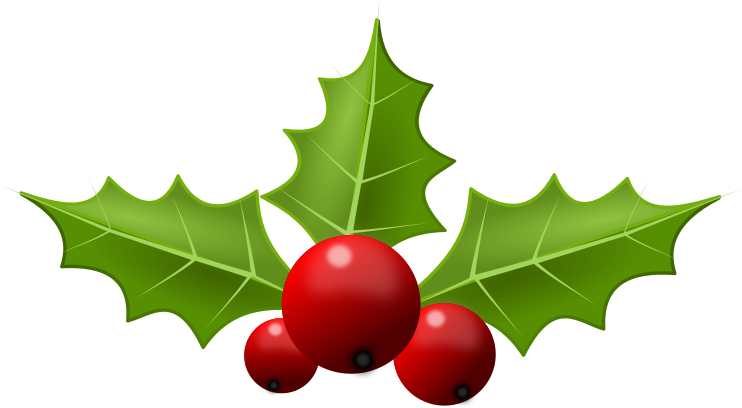
\includegraphics[width=.8\textwidth]{holly-berries-remix.png}
\end{center}


\newpage

\subsection{The compressing task}

Here is an example of a \emph{banko} board:

\begin{center}
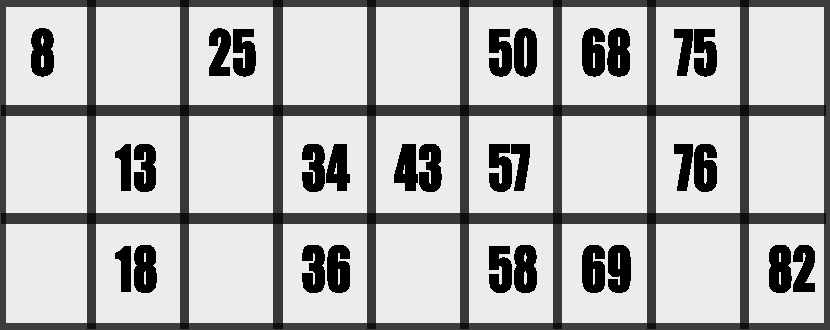
\includegraphics[width=.99\textwidth]{bankoplade.pdf}
\end{center}

This is a Danish game, similar to Bingo.  There are important rules for banko
boards.  Here they are\footnote{Nils Andersen.  Hvor
mange bankoplader er der?  2003.\\
\tiny{\url{http://sprutskalle.dk/blog/wp-content/uploads/bankoplader.pdf}}}:

\begin{itemize}
\item We use the numbers from 1 to 90, both inclusive.
\item A board has 3 rows and 9 columns.
\item A board has 15 different numbers and 12 empty fields.
\item There is at least one number in each column and exactly five numbers in
each row.
\item The first column (from the left), called $s_0$, can have the numbers $1$
to $9$.  The last column, called $s_8$, can have the numbers $80$ to $90$.  Each
column $s_n$, where $1 \leq n \leq 7$, can have the numbers $10n$ to $10n + 9$.
\end{itemize}

\textbf{Subtask 0:} Verify that the given example validates according to the
five requirements.

\textbf{Subtask 1:} Invent an algorithm for compressing a banko board
efficiently, i.e., represent it in few bits (without loss of information!).


\newpage

\subsection{The fun task}

% The Collatz conjecture

Here is a function for an arbitrary number $n$:
\begin{align*}
f(n) = \begin{cases}
n/2 &\text{if }n\text{ is even}\\
3n + 1 &\text{if }n\text{ is odd}\\
\end{cases}
\end{align*}
For example, $f(10) = 5$ and $f(7) = 22$.

Here is a sequence -- based on the function $f$ -- that starts with an arbitrary
number $n$:
\begin{align*}
a_i = \begin{cases}
n &\text{for }i = 0\\
f(a_{i - 1}) &\text{for }i > 0\\
\end{cases}
\end{align*}
If we e.g. set $n = 12$, we get the sequence
$a_0 = 12, a_1 = 6, a_2 = 3, a_3 = 10, a_4 = 5, a_5 = 16, a_6 = 8, a_7 = 4, a_8
= 2, a_9 = 1$.  We stop showing a sequence when it reaches the number $1$, since
$1$ is a pretty number, and since $f(f(f(1))) = 1$ (show this), so in any case
it will repeat at this point.

\textbf{Your task:} Prove or disprove the following conjecture:
\begin{quote}
No matter what initial number $n$ is chosen, the sequence will always reach the
number $1$.
\end{quote}

\textbf{\emph{Note: There is a free bottle of snaps to the first person who
finds a correct solution to this problem and brings it to the bar!}}
